\chapter*{Progress Report}
Feel free to contact me \\
0448 226 495 \\
michael.jurasovic@tasnetworks.com.au

\section{Project aims}
The aim of this project is to build upon existing research and develop a load forecasting system which can predict future load based on weather, holiday periods, car movement, and other factors. 
Bruny Island and the NAC will be used as a case study. 
The forecasting system is expected to be equally applicable to any power system network.
\\
Specifically, the system will have the following properties:
\begin{itemize}
	\item The system will produce a forecast up to 24 hours in the future in 15- to 60-minute intervals. This will be a rolling forecast that can be re-calculated at any time.
	\item The forecast will be able to begin from any point time.
	\item The forecast will predict load in kVA at each interval.
	\item The forecast system will be aimed at predicting aggregate load at the feeder level. That is, between approximately 0.5 and 10MVA.
	\item The forecast system will be especially tuned to predict load during holiday periods.
\end{itemize}
\par
A neural network based model is being considered to achieve these aims.


\section{Summary of work completed}
All work completed has been integrated into a single software package that will allow all methods and variations of methods to be compared. This has constituted the majority of the work.

Analysis has been performed on the available data (load, weather, traffic) to investigate patterns, the beginning of which has been written up in section \ref{bruny-data-analysis} of the draft thesis.
Weekly and yearly repetition has been observed in both the load and car movement data - indicating that a naive similar day selection approach could be effective.

It was hypothesized that if two load profiles have a high correlation coefficient, then their weather profiles will also have a high correlation coefficient and could be used to identify similar days, similar to the approach implemented by \cite{Bennett2014}.
A highly parallelised GPGPU approach allowed this theory to be disproven in a practical amount of time.
This may be revisited using load profile features rather than the full load profile itself.

Clustering of load profiles was performed based on the morning and afternoon peak magnitudes and prominences, and the total energy usage.
This did not produce significant insights into the data - it merely highlighted the already understood differences between holidays and normal days.

The inspiration for using a sequence to sequence (S2S) recurrent neural network (RNN) was the paper by \cite{Marino2016} whose approach was elegant and effective, and was further supported by \cite{Bianchi2017} and \cite{Kong2017}.
This approach has been implemented and found to be consistent with the papers, and has now been expanded with the following:
\begin{itemize}
	\item Bidirectional recurrence \citep{Schuster1997}.
	\item Gated recurrent unit cell \citep{Cho2014}.
	\item Bahdanau attention \citep{BahdanauCB14}.
	\item Dropout \citep{srivastava14a}.
	\item Discretization of output vectors to allow for cross entropy loss and indication of uncertainty in the output.
\end{itemize}

The state of the art neural machine translation architecture was implemented for load forecasting \citep{Vaswani2017} and found to perform better than the S2S RNN. The only related published work is by  \cite{Song2017} who used the transformer architecture for classification of time series in a medical context.

Various "low hanging fruit" approaches have been implemented to make the forecasting system more accurate, none of which have resulted in improvements:
\begin{itemize}
	\item Training individual systems for each hour of the day.
	\item Adjusting the training process such that days with high load are trained on equally as often as days with normal and low load.
	\item Training on only days with large load.
	\item Weighting of the neural network loss function to prioritize large load forecasts.
	\item Using data of different periods including 5, 20, and 30 minutes.
\end{itemize}
It is my opinion that this lack of improvement from simple tweaks speaks to the versatility and robustness of the selected neural network architecture.
I expect to discuss this in more depth in the final thesis.

\section{Guide to draft thesis}
The thesis is structured into three chapters:
\begin{enumerate}
	\item \textbf{Introduction} - this chapter introduces and defines the problem being addressed, provides background on load forecasting in general, and goes over a number of recently published approaches. 
	At this stage of the draft thesis, this section contains a lot of detail that will be moved to chapter \ref{ana-meth}.
	This section will be revised in such a way that it is approachable for a technical reader with no background in load forecasting.
	\item \textbf{Analysis and Methodology} - this chapter expands on the introduction and evaluates empirically the performance of various architectures.
	At this stage, the architectures that will be finally used it still being decided.
	This will likely be finalised once their performance with similar day features is evaluated.
	\item \textbf{Case Study} - this chapter will present a case study of the load forecasting system to Bruny Island.
	At this stage, it only has the beginning of the data analysis for Bruny Island completed.
	The data analysis section currently rambles quite a lot - it will be heavily revised.
\end{enumerate}

The thesis is currently using Harvard style referencing because I find this easier to work with when I am editing.
This will be changed to IEEE style for the final thesis.

\section{Plan for completion}
A software package that is able to perform and evaluate load forecasting using all techniques investigated has been developed and has been working reliably.

The next step in this project is to implement similar day selection and use the similar days as additional inputs to the forecasting model.
Analysis of the available data has shown that there is significant correlation between load profiles with one week and one year delays.
This observation will be used to implement an initial basic similar day selection technique.
This is a well established technique and is expected to produce significant improvements.
Once this has been implemented it will be further refined if deemed necessary.

The software package will then be extended to produce more informative graphs to simulate what predictions it would make if it were running in the past.
This visualisation will be key in determining if the system is adequate to be implemented in production, as well as evaluating the performance in general.

After this stage the software will be extended to work with the current NAC forecasting software. 
Access has been given to the source code behind this and initial review indicates that the system is quite clean and simple, and so will be unlikely to present an issue.

The final stage will be to comprehensively evaluate the performance of the system against other forecasting methods.
These other forecasting methods will be implemented in the developed software package in order for this to work.

If there is time, I would like to try to extend this work and investigate the use of a differentiable function that is able to select similar days from the past.
This would require quite a bit of additional research, but I suspect it could be implemented by applying existing attention mechanisms used in computer vision, especially those used in neural image captioning.

An updated gantt chart is attached.


\section{Comments on progress}
This project is behind schedule.
This is mainly a result of the lack of improvement from "low hanging fruit" attempts at increasing accuracy - it was expected that these would produce enough improvement for the project to move forward to testing and thorough evaluation.
As a result, the project will need to miss out on one round of on-line evaluation in the NAC.
This is not expected to be a severe handicap for the project, as three on-line evaluations were scheduled which was quite optimistic.

The developed software package is becoming increasingly complex and as such presents a risk to the project.
This risk will be mitigated through adherence to basic software design principles \citep{Haoyu2012}.

In the original project plan it was mentioned that computing resources may become a bottleneck.
This occurred and was mitigated through acquisition of higher performance hardware.
It is unlikely this will be an issue in the future.

I am confident this project will be completed on time.


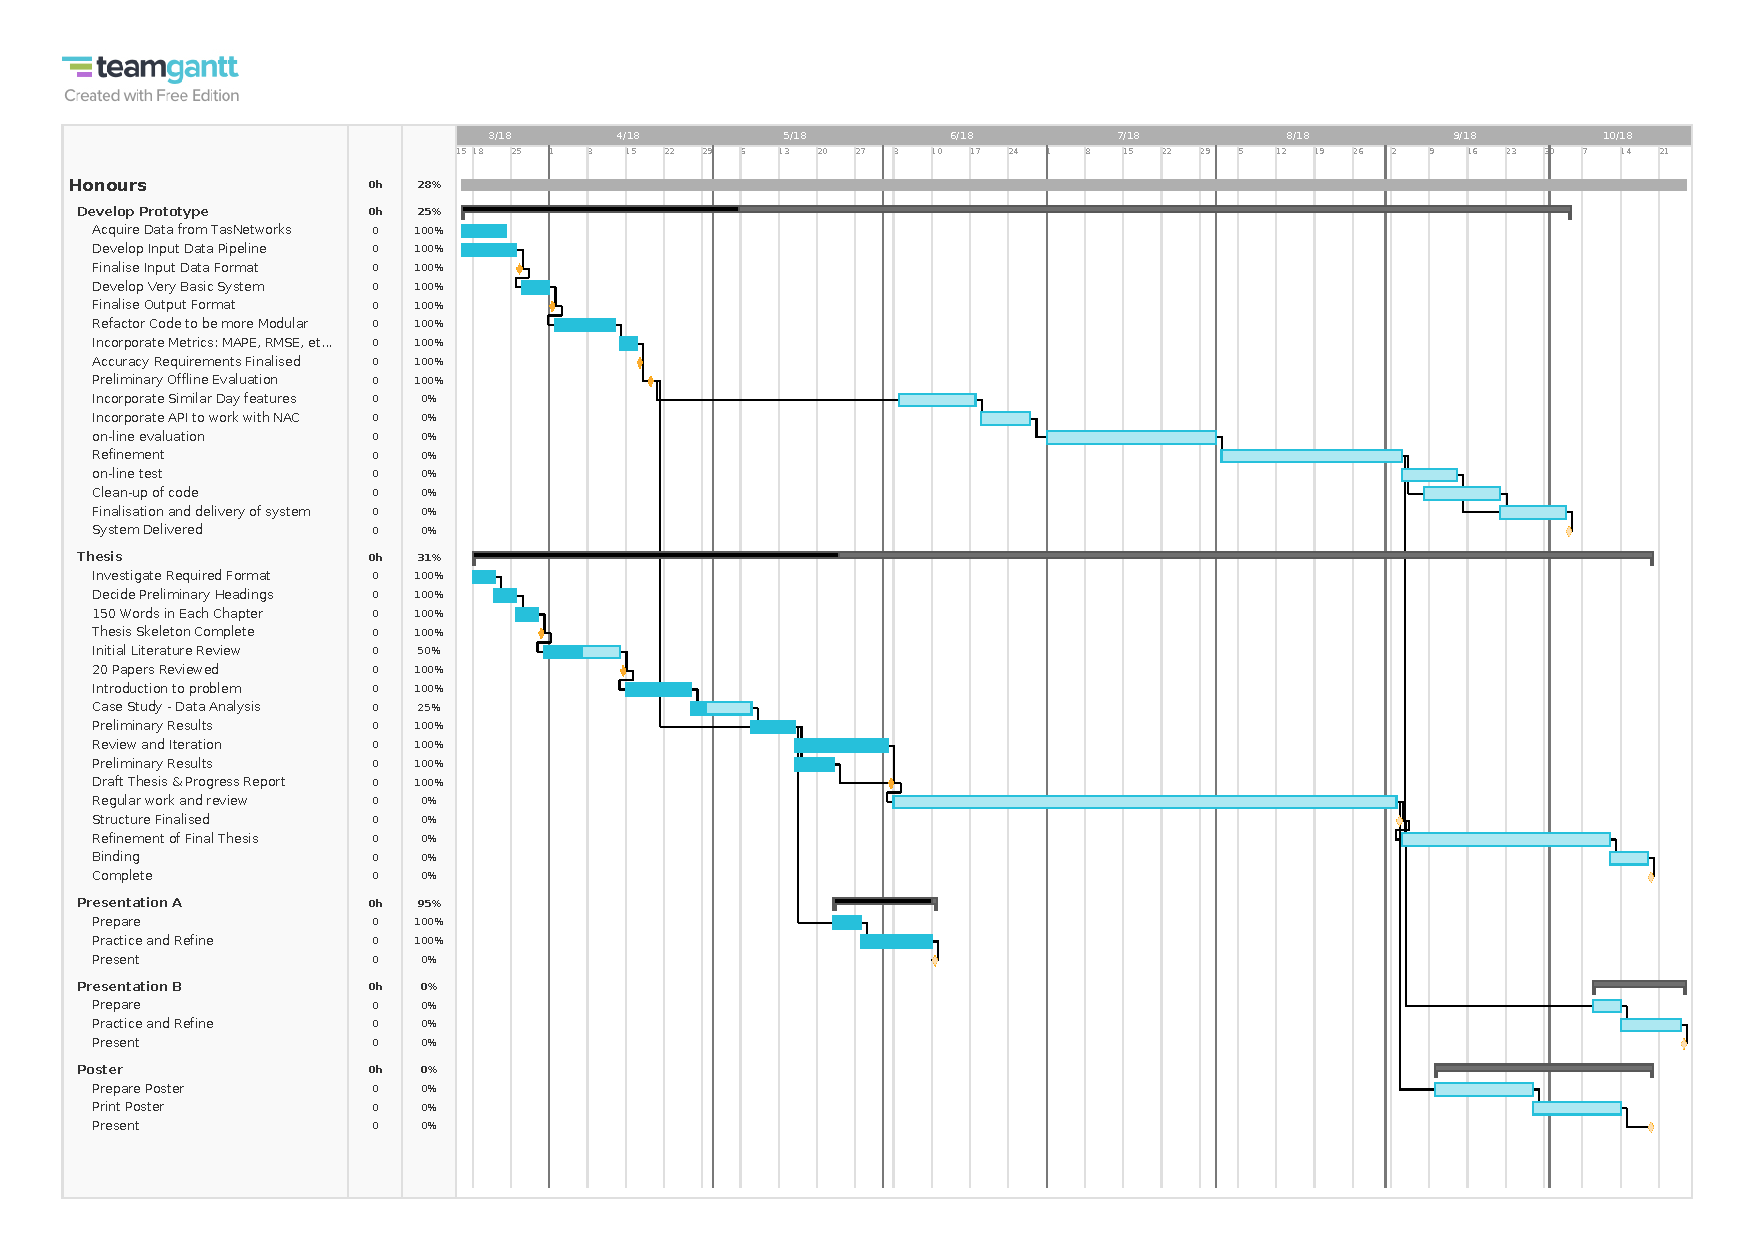
\includepdf[pages={1}, angle=90, pagecommand={\thispagestyle{plain}}]{pdf/gantt-progress-report.pdf}